\documentclass{IEEEcsmag}

\usepackage[colorlinks,urlcolor=blue,linkcolor=blue,citecolor=blue]{hyperref}

\usepackage{upmath}
\usepackage{comment}
\usepackage{graphicx}

\usepackage[usenames,dvipsnames,svgnames,table]{xcolor}
\definecolor{dkgreen}{rgb}{0,0.6,0}
\definecolor{mauve}{rgb}{0.58,0,0.82}
\definecolor{light-gray}{gray}{0.88}

\usepackage{listings}
\lstdefinestyle{agree}
{frame=none,
  basicstyle=\ttfamily,
  language=ML,
  aboveskip=3mm,
  belowskip=3mm,
  showstringspaces=false,
  columns=flexible,
  numbers=none,
  numberstyle=\tiny\color{gray},
  commentstyle=\color{dkgreen},
  stringstyle=\color{mauve},
  breaklines=false,
  breakatwhitespace=true,
  tabsize=2,
  linewidth=1.7\linewidth,
  morekeywords={eq, bool, guarantee, assume, true, false, pre, not, and, or, property, const}
}

% for diagram in synthesis.tex

\usepackage{tikz}
\usetikzlibrary{shapes}

\newcommand{\briefcase}{BriefCASE}
\newcommand{\hamr}{HAMR}
\newcommand{\selFour}{seL4}
\newcommand{\figref}[1]{Fig.~\ref{#1}}
\newcommand{\agree}{AGREE}
\newcommand{\splat}{SPLAT}
\newcommand{\resolint}{Resolint}
\newcommand{\resolute}{Resolute}

\jvol{XX}
\jnum{XX}
\paper{XX}
\jmonth{XX/XX}
\jname{Security \& Privacy}
\pubyear{2022}
\newtheorem{theorem}{Theorem}
\newtheorem{lemma}{Lemma}

\setcounter{secnumdepth}{0}

\begin{document}

%\sptitle{Department: Head}
%\editor{Editor: Name, xxxx@email}

\title{Cyber Assured Systems Engineering at Scale}
%\title{Cyber-Resilient Systems Engineering at Scale}

\author{Darren Cofer, Isaac Amundson, Junaid Babar, David Hardin, Konrad Slind}
\affil{Collins Aerospace}

\author{Perry Alexander}
\affil{University of Kansas}

\author{John Hatcliff, Robby}
\affil{Kansas State University}

\author{Gerwin Klein}
\affil{Proofcraft and UNSW Sydney}

\author{Corey Lewis}
\affil{UNSW Sydney}

\author{Eric Mercer}
\affil{Brigham Young University}

\author{John Shackleton}
\affil{Adventium Labs}

\markboth{Department Head}{Paper title}

\begin{abstract}
Formal methods tools that provide mathematical proof of system properties
have improved dramatically in their power and capabilities. Our team has developed a model-based systems
engineering environment that integrates formal methods at all levels of system design.
Our methodology and tools enable systems engineers to address
cybersecurity concerns early in the development of complex high-assurance systems.
\end{abstract}

\maketitle


%Darren, David? Budget: 1 column
%Introduction
\chapterinitial{Aerospace systems engineers} are currently given few
development tools to understand and mitigate 
potential cybersecurity vulnerabilities.  Typically, they must rely on
process-oriented checklists and guidelines. Cyber vulnerabilities
are often discovered during penetration testing late in the
development process. Worse yet, they may be discovered
only after the product has been fielded, necessitating extremely
expensive and time-consuming remediation. This is not a
sustainable development model.

Fortunately, formal methods tools have advanced to the point that they can 
be used to address cybersecurity and cyber-resiliency design challenges
on real high-assuance systems at industrial scale.  
Our application domain is avionics and aerospace systems in general.  
They are typically large, real-time cyberphysicial systems with the added 
complexities of performing safety-critical tasks and being exposed to 
a wide variety of cyber threats.  Furthermore, they are subject 
to intense regulatory scrutiny due to the certification requirements of this domain. 

In previous work on the High-Assurance Cyber Military Systems (HACMS) project \cite{HACMS}
we demonstrated that formal methods could be used to dramatically improve the 
cyber-resiliency of real aircraft, including an unmanned military helicopter.  Our current
work is focused on automating the capabilities that we prototyped in the HACMS project
and extending the reach and scale of the formal methods design and verification approach.  

To this end, we have developed a model-based systems engineering (MBSE) 
environment that allows engineers to address a range of properties and 
manage system complexity through compositional analysis, integrating formal methods
at all levels of the design process.  MBSE processes use model as the primary vehicle for 
communication among the parties tasked with designing the system and as the primary 
design artifacts for requirements, verification, and code generation.  

Our tools are based on the 
Architecture Analysis and Design Language (AADL) and extend the Open Source
AADL Tool Environment (OSATE) \cite{OSATE}.  The tools are specifically designed 
to bridge the gap between a user-level modeling language accessible to systems 
engineers and the highly specialized, formally verified code that implements the operating system (OS)
kernel and other high-assurance components.   

By using these tools to build real avionics systems, we show 
that current formal methods tools are practical, effective, and scalable to significant 
high-assurance applications in the aerospace industry.  


\section{INNOVATIONS}
%Darren -  Budget: 1 column
%Innovations

MBSE environment for high-assurance systems, providing access to FM tools at every level, integrating assurance evidence for co-evolving design and associated evidence.

\begin{enumerate}
\item Semi-automated architectural design patterns to address cyber-resiliency requirements, including synthesis of high-assurance components
\item MBSE environment that leverages seL4 security guarantees and makes this accessible
\item Co-evolution of system design and certification evidence/artifacts, organized by assurance argument
\item Integration of formal methods throughout the workflow (or is this part of one of the other innovations?)
\end{enumerate}

As part of the DARPA Cyber Assured Systems Engineering (CASE) program,
our team has developed design, analysis, and verification
tools that enable systems engineers to design-in cyber-resiliency
for complex cyber-physical systems. We have produced a prototype
Model-Based Systems Engineering (MBSE) environment called
BriefCASE which is based on the Architecture Analysis and Design
Language (AADL). BriefCASE extends the Open Source AADL
Tool Environmnet (OSATE) to add new design, analysis, and code
generation capabilities targeted at building cyber-resilient systems.
BriefCASE provides access to two analysis tools (GearCASE 
and DCRYPPS) that can examine AADL models to detect potential
cyber vulnerabilities and suggest requirements for mitigation.
A library of architectural transforms guides systems engineers
through automated model transformations that modify the
architecture to address these requirements, possibly inserting new
high-assurance components into the system. Implementations for
these new high-assurance components are synthesized from formal
specifications using the Semantic Properties for Language and
Automata Theory (SPLAT) tool. Formal verification that the
transformed system model satisfies its cyber requirements is accomplished
via model checking using the Assume Guarantee Reasoning
Environment (AGREE). Cyber-resilient code implementing the
verified model is automatically generated using the High Assurance
Modeling and Rapid Engineering for Embedded Systems (HAMR)
toolkit. If desired, this code can be targeted to the formally
verified seL4 secure microkernel.
A novel aspect of our approach is the use of an assurance argument
embedded in the architecture model itself to capture and
document the design decisions made during this process, along
with associated rationale.


\section{EXAMPLE}
%Eric?  Budget: 1 column
%Motivation
\begin{figure*}
	\begin{center}
	  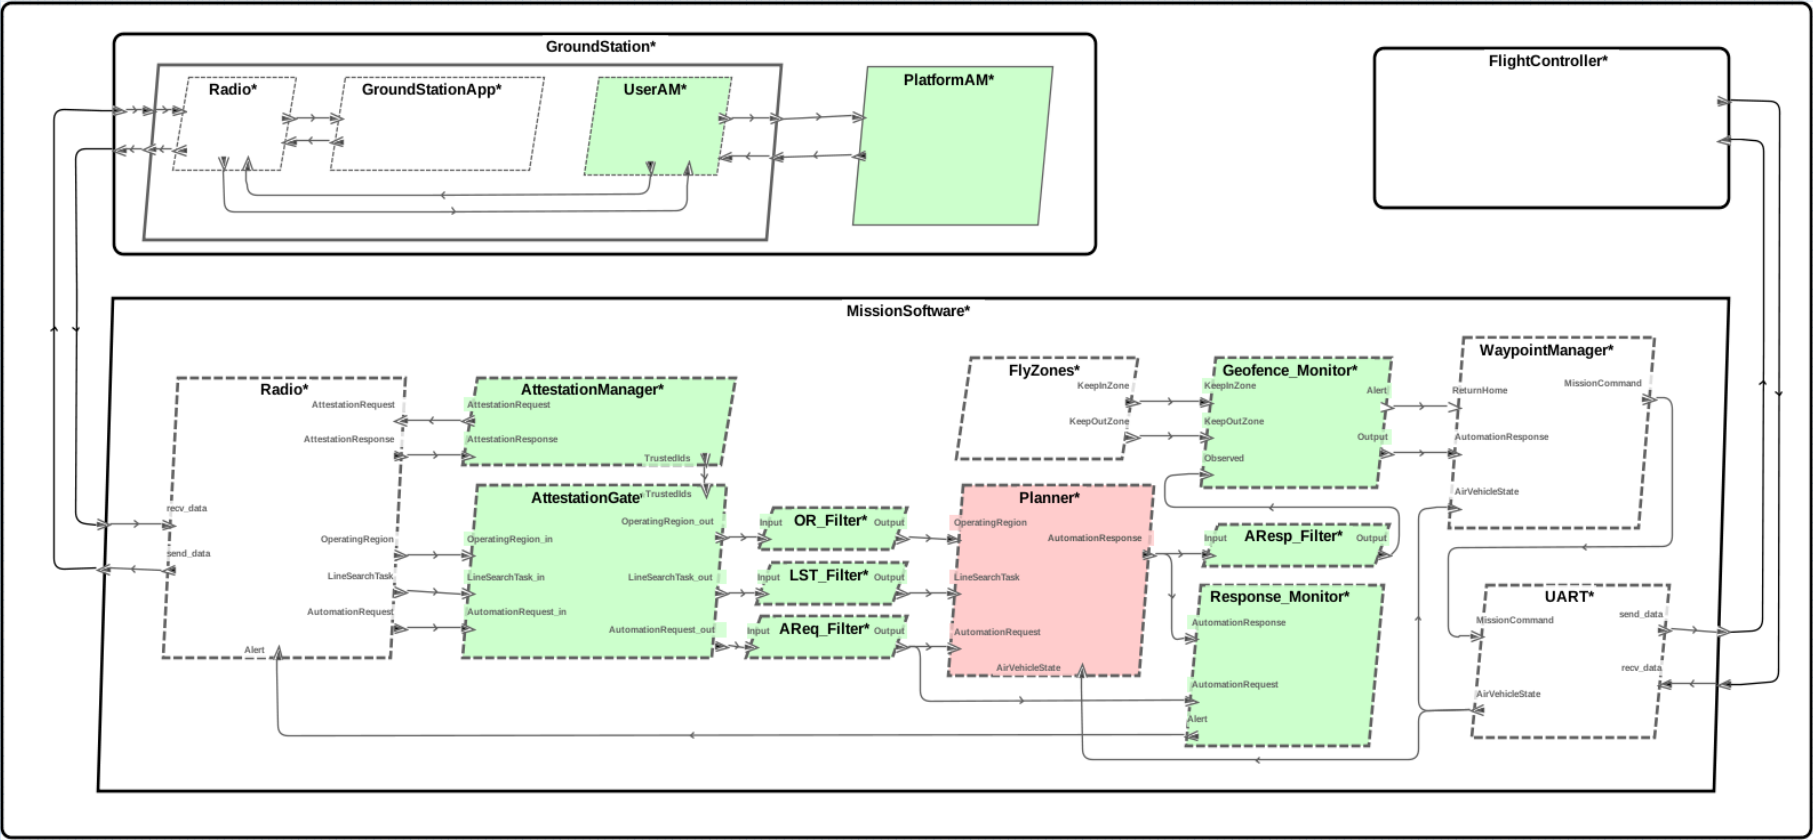
\includegraphics[width=\textwidth]{./figs/sw-hardened.png}
  \end{center}
	\caption{Cyber-resilient software architecture for UAV surveillance system. MAKE NAMES BIGGER} 
	\label{fig:sw-hardened} 
\end{figure*}

\figref{fig:sw-hardened} is a model-based design in the AADL OSATE tool of a cyber-hardened software
system for an autonomous UAV for surveillance.
The original \emph{unhardened system} consists of four components: the radio to communicate with a
remote ground
station (\emph{Radio}), mission planning automation (\emph{UxAS}), waypoint metering
(\emph{WaypointManager}), and a UART to talk to the flight controller (\emph{UART}).

\briefcase\ integrates four key formal methods in the model-based engineering workflow:
assume-guarantee verification (\agree), synthesis of high-assurance components (\splat), synthesis
of inter-component communication (\hamr), and the \selFour\ verified microkernel.
Each component in the unhardened system, and the interface for the top-level software component, is
formally specified with an AGREE contract stating assumptions on inputs and guarantees on outputs
under the assumptions.
\agree\ proves the unhardened implementation obeys the composition of these contracts. 

Cyber-threat analysis (GearCASE and DCRYPPS) identifies the ground station and the planning
automation services as primary cyber threats to the system.
Seven new cyber requirements are added to the unhardened system that require ground station
certification, message integrity, and monitoring.
The existing contracts in the unhardened system are strengthened to reflect these new requirements.
\agree\ proves the unhardened system under these contracts fails verification. 

Design engineers use \briefcase\ to transform the unhardened system to that in
\figref{fig:sw-hardened} by inserting high-assurance components.
\emph{Attestation} proves the identity of trusted ground stations (\emph{AttestationManager}) while
the \emph{gate} only passes messages from trusted sources (\emph{AttestationGate}).
\emph{Filters} only pass well-formed messages (\emph{OR\_Filter}, \emph{LST\_Filter},
\emph{AReg\_Filter}, and \emph{AResl\_Filter}).
\emph{Monitors} alert to suspicious behavior such as missions that enter keep-out zones or leave
keep-in zones (\emph{Geofence\_Monitor}) or unrequested missions from automation
(\emph{Response\_Monitor}).
The interface behavior of these high-assurance components, with the exception of attestation, is
specified with assume-guarantee contracts (e.g., a filter makes no assumptions on input and only
passes input that is well-formed).
\agree\ proves the hardened system ensures the added cyber requirements.

The \selFour\ target platform requires a static schedule that is provided in the model.
A transformation on the \agree\ contracts incorporates that schedule into the verification model.
\agree\ proves the scheduled hardened system also ensures cyber requirements.
The model is further refined to move the attestation and mission planning services into separate
virtual machines inside the microkernel.

\resolint\ certifies the hardened model is ready for synthesis.
\splat\ synthesizes high-assurance components from their \agree\ contracts to the target platform.
It includes proof certificates that the binaries have assumptions that are no stronger than those on
the original contracts and guarantees that are no weaker than those on the original contracts (e.g.,
safe substitution).
\hamr\ synthesizes all the inter-component communication primitives from the AADL model.
That synthesis includes a proof certificate that the resulting communication channels defined in
\selFour\ are only those defined in the AADL model.

\resolute\ builds an assurance case for the entire system.
That assurance case includes evidences for every requirement including proof certificates from
\agree, \splat, and \hamr.


\section{BRIEFCASE WORK FLOW}
%Darren write a brief intro -  Budget: 0.5 column
%\cite{OSATE}
%Work Flow

%Describe the BriefCASE work flow and tools.

% Copied from DESTION paper
The BriefCASE environment provides systems engineers with a workflow and tool support for developing
products with inherent cyber-resiliency. 
\remove{In this section we provide an overview of the design, analysis, and code generation tools and how they can be used
to implement high-assurance systems.  
}

%BriefCASE is predicated on an MBSE process, in which models are the primary vehicle for
%communication and understanding among the parties tasked with designing the system. Furthermore,
%MBSE models are the primary design artifacts used for analysis, verification, testing, and code
%generation.
The  workflow starts with the development of a baseline AADL model of the system architecture
focusing on the desired functionality. This model can be analyzed using any of the existing AADL 
tools (e.g., resource usage, information flow, latency) to determine whether it is acceptable.
BriefCASE integrates additional tools that analyze the architecture model for cybersecurity vulnerabilities and
generate requirements that, when addressed, will mitigate those vulnerabilities.
These requirements are imported into the model and may be addressed using a 
collection of automated model transforms. As requirements are addressed in the design, an assurance case is updated with
corresponding evidence, computed directly from the model or by supporting analysis tools.  
Code implementing new high-assurance components as well as communication and execution infrastructure
is generated from the model along with associated assurance evidence.  

The following sections describe each step of the workflow in more detail. 

%development process outputs, necessary
%to support the claim. In this manner, the assurance case is co-developed alongside the system
%design, and can be automatically evaluated throughout development.


\subsection{Requirements}
%Isaac, Junaid -  Budget: 1 column
%\cite{gearcase2020} \cite{dcrypps2019}
BriefCASE provides access to two analysis tools (GearCASE~\cite{gearcase2020} and
DCRYPPS~\cite{dcrypps2019}) that can examine AADL models to detect potential cyber vulnerabilities
and suggest requirements for mitigation.
%
Systems engineers are %then
presented with a requirements management interface
(top pane in Figure~\ref{fig:req-mgmt}) for viewing the generated requirements and importing them into the model
so they can be addressed. The interface enables engineers to select the requirements they wish to
import and assign them unique identifiers, or omit them with rationale. A document listing the omitted
requirements and rationale is maintained and may be a required development artifact for some
certification domains. 

\begin{figure*}[h]
	\centering
	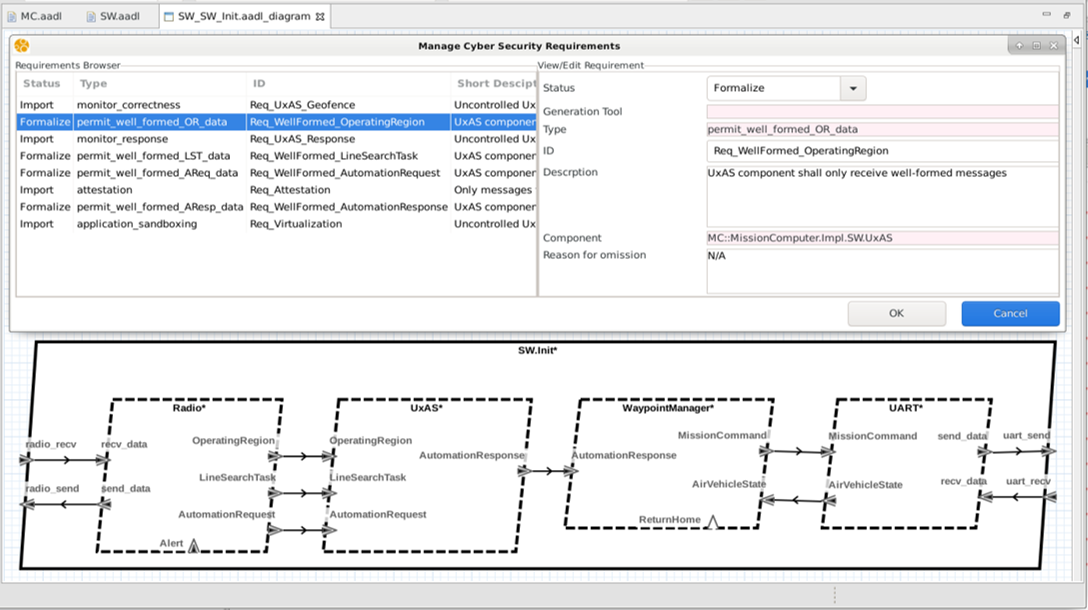
\includegraphics[width=\textwidth]{figs/req-mgmt.png}
	\caption{\briefcase \ requirements management interface.} 
	\label{fig:req-mgmt} 
\end{figure*}

Some requirements can also be formalized as assume-guarantee contracts
added to the AADL model, enabling formal verification. 
Such a requirement will be imported into the model with with an associated formal
contract.

A BriefCASE project contains a repository for requirements. Imported requirements are represented 
as assurance case goals to be satisfied. For example, one of the requirements for well-formed 
messages (selected in \figref{fig:req-mgmt}) is imported as the following goal:

\noindent
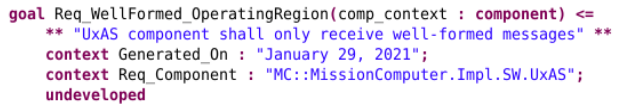
\includegraphics[width=1\columnwidth]{figs/req-wellformed-or.png}

% shown in \figref{fig:req-wellformed-or}.
\noindent
% Initially, the goal is marked {\em undeveloped} and does not contain any evidential statements.  
% These will be added as the design is updated to address this requirement.  
The goal is marked {\em undeveloped} initially.
Evidential statements are added to the goal as
the design is updated to address this requirement.

%for Resolute to evaluate in order to determine whether the goal has been satisfied. Running Resolute
%at this time will therefore produce a failed assurance case.

%\begin{figure}[h]
%	\centering
%	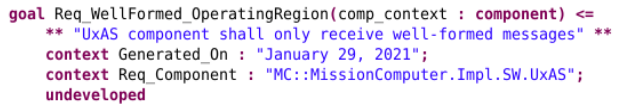
\includegraphics[width=1\columnwidth]{figs/req-wellformed-or.png}
%	\caption{Requirement for well-formed messages.  NEEDED? CONVERT TO TEXT?} 
%	\label{fig:req-wellformed-or} 
%\end{figure}


\subsection{Cyber Transforms}
%Isaac -  Budget: 1 column
To address the new requirement, the architecture will need to be transformed in such a way as to harden the design against the vulnerability.
BriefCASE provides a library of model transformations for addressing common cyber vulnerabilities.  Currently, the following transformations are supported:

\begin{itemize}
	\item Attestation
	\item Filter
	\item Monitor
	\item Virtualization
	\item Proxy
	\item Switch
	\item seL4
\end{itemize}  

The transformations are automated by the tool, resulting in a hardened model that is correct-by-construction.  
For example, ensuring a component only receives well-formed messages can be accomplished by the insertion of a high-assurance filter.  The BriefCASE Filter transform wizard (Figure~\ref{fig:filter-wiz}) enables the configuration of filter component properties, including the filter behavioral specification, which is represented in the AGREE language.

\begin{figure}[h]
	\centering
	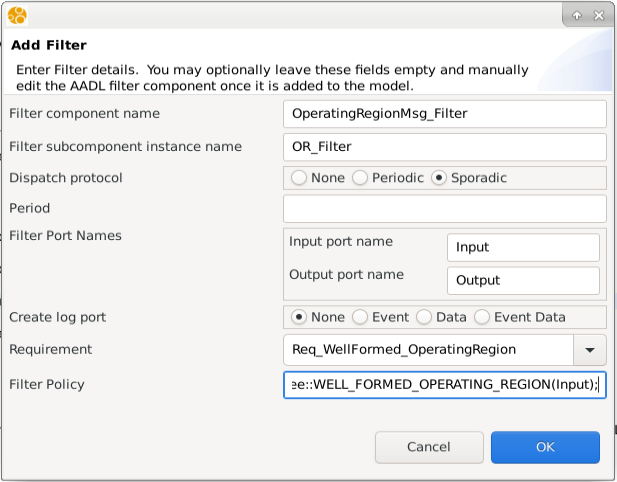
\includegraphics[width=0.7\columnwidth]{figs/filter-wiz.png}
	\caption{Filter transform wizard.} 
	\label{fig:filter-wiz} 
\end{figure}

BriefCASE inserts a new filter component into the model, sets the component properties, and establishes the appropriate connections to source and destination components. The filter specification is inserted into an AGREE annex, enabling both formal analysis of the model as well as providing the behavioral specification for a provably correct synthesis of the component implementation via the SPLAT plugin.

The transformation also updates the Resolute goal with new evidential statements pointing to evidence that the model has indeed been hardened against the vulnerability and the requirement has been satisfied (as shown in Figure~\ref{fig:resolute-add-filter}).
For example, the \texttt{add\_filter} strategy is included in a library of built-in Resolute transform rules and provides Resolute with the logical instructions for evaluating if the top-level goal has been satisfied.
The \texttt{add\_filter} definition (shown in Figure~\ref{fig:resolute-add-filter}) includes the following sub-goals: 
\begin{itemize}
	\item \texttt{filter\_exists} - the filter component exists in the model
	\item \texttt{filter\_not\_bypassed} -  there is no alternate pathway in the model that can bypass the filter
	\item \texttt{filter\_implemented\_correctly} - the filter has been implemented correctly
\end{itemize}


\begin{figure}[h]
	\centering
	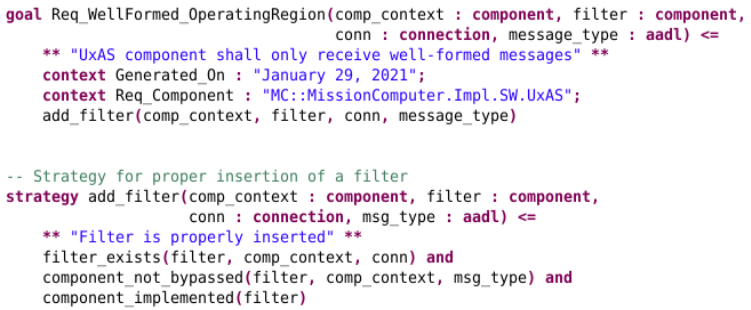
\includegraphics[width=1\columnwidth]{figs/resolute-add-filter.png}
	\caption{Updated well-formedness claim.} 
	\label{fig:resolute-add-filter} 
\end{figure}

The first two sub-goals are supported by evidence obtained by examining the structure of the model, while the last is determined by examining the output of the synthesis tool.  This approach follows the model-based decomposition pattern based on~\cite{model-based-decomposition}, and is representative of all BriefCASE transform assurance strategies.
If at a later time during development the model is inadvertently altered in a way that renders the transformation ineffective, Resolute will be unable to substantiate the evidential statements, and therefore produce a failing assurance case.

The third subgoal is satisfied by SPLAT.  SPLAT not only generates the  implementation code for high-assurance components such as filters, monitors, and gates, but it also produces a proof that this code correctly implements its AGREE specification.  
Resolute uses the existence of the SPLAT proof as evidence that the component was implemented correctly.

\subsection{Compositional Analysis}
%Junaid -  Budget: 1 column
%\cite{case-models-2021}
% Compositional Analysis

The Assume Guarantee Reasoning Environment (AGREE) is a compositional, assume-guarantee-style model
checker for AADL models \cite{compositional-analysis-agree}. AGREE attempts to prove properties about one layer
of the architecture using properties allocated to subcomponents. The composition is performed in
terms of assumptions and guarantees that are provided for each component. Assumptions describe the
expectations the component has on the environment, while guarantees describe bounds on the behavior
of the component. 

AGREE uses k-induction as the underlying algorithm for model checking.  AADL models and AGREE
contracts are first translated into the Lustre language, including verification conditions for consistency
and correctness of the contracts.  The model checker then attempts to find any model execution traces
that would violate these conditions using one of several Satisfiability Modulo Theories (SMT) solvers. 
If the model checker covers all reachable states in the model without finding a violation then the properties are proved. 

Once the system architecture has been modeled using AADL
and the component behavior is specified using \agree's assume-guarantee contracts,
we use the \agree{} model checker to verify the consistency of these contracts.

\begin{enumerate}
\item Component interfaces -- The output guarantees of each component must be strong enough to
satisfy the input assumptions of downstream components. 
\item Correctness of implementations -- The input assumptions of a system along with the 
output guarantees of its \emph{sub}-components must be strong enough to satisfy its output guarantees.
\end{enumerate}

For example, in \figref{fig:sw-hardened},
the input assumptions of the Waypoint Manager must be weaker than
the output guarantees of the Geofence monitor 
\textit{and} the output guarantees of the Mission Software must be inferrable from
its input assumptions combined with the output guarantees of its components.

This hierarchical strategy for reasoning about contracts,
or \emph{compositional analysis},
reduces the computational complexity of model checking
by breaking down the larger problem into more manageable fragments.
Verification of a system does not directly depend on the implementations of its components (or their sub-components),
but only on their contracts.  
In \figref{fig:sw-hardened}, each of the Mission Software components either contains subcomponents 
or has a corresponding source code implementation of its contract.  
Rather than reasoning monolithically about the interaction of all of these lower-level implementations, 
the compositional approach allows us to reason about each layer of the model separately.  
%More details on the use of composition to reduce verification complexity can be found in \cite{case-models-2021}.


\subsection{High Assurance Component Synthesis}
%% Konrad, Eric, Junaid -  Budget: 1 column
%% \cite{case-verified-filter} \cite{hardin-co-assurance}
%% \cite{formal-filter-synth-langsec} \cite{contiguity-types}
The correctness of the leaf-level components introduced by CASE
transformations resolves to the question of whether such a component
meets its \agree{} contract. This obligation is addressed by
\emph{formal synthesis}: given a sufficiently detailed formal
specification of component behavior, the \splat{} tool generates code
from it and also generates proofs showing that the generated code is
correctly compiled and meets its specification.

The formal languages that filters, gates, and monitors are generated
from include regular expressions, contiguity types
\cite{contiguity-types}, and Lustre \cite{lustre}. For each of these
languages, we have infrastructure (see Figure \ref{fig:synthesis})
that (a) translates formal specifications to code and (b) proves the
correctness of the translation using the HOL4 system
\cite{hol4:overview}. The generated code is \emph{CakeML}, a dialect
of Standard ML \cite{SML97} possessing a fully verified compiler
\cite{cakeml}.

\begin{figure}[h]
\begin{center}
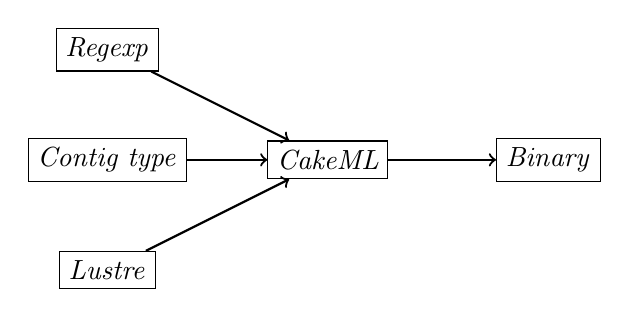
\begin{tikzpicture}[scale = 0.7]
\node (A) at (0,2) [shape=rectangle,draw]{\textit{Regexp}};
\node (B) at (0,0) [shape=rectangle,draw]{\textit{Contig type}};
\node (C) at (0,-2) [shape=rectangle,draw]{\textit{Lustre}};
\node (D) at (4,0) [shape=rectangle,draw]{\textit{CakeML}};
\node (E) at (8,0) [shape=rectangle,draw]{\textit{Binary}};
\draw [->,thick] (A) to (D);
\draw [->,thick] (B) to (D);
\draw [->,thick] (C) to (D);
\draw [->,thick] (D) to (E);
\end{tikzpicture}
\end{center}
\caption{\splat{} Verified Synthesis Path.\label{fig:synthesis}}
\end{figure}

Regular expressions and contiguity types are formalisms well-suited
for expressing classes of constraints on the data passed in
messages. Thus they provide a useful basis for expressing
filters. Regular expressions compile to efficient finite state
automata, generating a correctness proof along the way
\cite{case-verified-filter}.  We have also synthesized regular
expressions to hardware using this proof-producing
technique \cite{formal-filter-synth-langsec}.
Contiguity types can capture more complex
data formats, including variable-length arrays and union structures;
this level of expressiveness was needed to handle the messages of
UxAS. We deploy a verified contiguity-type based parser generator
\cite{contiguity-types} to decode and check the wellformedness of
such serialized data.

Gates and monitors can require arbitrarily complex computations for
their work; hence we also support code generation from Lustre. We have
formalized the semantics of Lustre and are using it as the basis for a
formal translation to CakeML.

Since code generated from \splat{} is deployed as a scheduled thread
in a real-time environment, there are two aspects to consider: (1)
correctness of a `one shot` thread execution (discussed above), and
(2) correctness of the perpetual re-execution of the thread. How to
model the latter and prove relevant properties is discussed in
\cite{johannes:repeat}.


\subsection{Remote Attestation}
%Perry -  Budget: 1 column
%\cite{copland-attestation} \cite{copland-verification}
Semantic remote attestation is a technique for  establishing
trust in software running on a non-local computer.  
An appraiser requests an attestation from
a target, receives evidence in response to the request, and appraises
the evidence to determine
trust~\cite{Coker::Principles-of-R}. Because
remote attestation does not require modification of its measurement
target, we utilize it to establish trust in legacy software
that cannot otherwise be verified.  We construct a verified remote
attestation infrastructure around the legacy target that generates
run-time and boot-time evidence.

In the UAV example, we wish to ensure that the aircraft will only accept
commands from trustworthy (non-compromised) ground stations.  
Our approach adds three attestation managers to the seL4-based
architecture in \figref{fig:sw-hardened}.  Each attestation
manager executes protocols specified by Copland~\cite{Ramsdell:2019aa}
phrases.  Copland is a formal specification language designed for
writing attestation protocols that are both verifiable and executable.
The attestation managers themselves are written and verified using
CakeML and Coq.

The \emph{AttestationManager} on the Mission Computer makes
attestation requests and appraises the results.  A protocol request and nonce are
sent to the remote target (in this case, the Ground Station), 
evidence is returned, and results appraised to
determine trust.  If the appraisal is successful, the identifier for the 
target is added to a list of trusted computers whose messages 
will be allowed to pass through the \emph{AttestationGate}.  
%The AttestationManager then communicates appraisal
%results to the platform communicating with the remote target.  In this
%way the platform appraises a remote target before trusting it to
%behave as expected.
Attestation can be requested periodically if warranted by the anticipated
threats against the remote system.  

Two other attestation managers must be added on the Ground Station.  
The Ground Station software has been modified to run in a Linux virtual 
machined hosted on \selFour.  
The UserAM runs as a Linux process on this virtual machine.  Its
responsibilities include responding to attestation requests from the UAV, 
measuring the Ground Station application software, and requesting
attestations from the Ground Station platform (the Linux kernel).  When the UserAM receives an
attestation request it responds by executing an attestation protocol
that measures the application, requests measurements from the
PlatformAM, signs the result, and generates a nonce from the request.  The
resulting evidence package is returned to the requesting appraiser on the UAV.

Because the UserAM runs as a Linux process, it cannot be
trusted \emph{a priori}.  A PlatformAM is introduced to perform an
attestation of the Linux kernel (and the UserAM).  The PlatformAM runs as a
\selFour \ component outside of the Linux virtual machine 
separated from the Linux kernel.  \selFour's guaranteed
separation properties provide assurance that the PlatformAM cannot be
compromised by other platform software.  The PlatformAM only
responds to requests from the UserAM and similarly runs a protocol
that produces signed results.

Using the remote attestation system to harden a platform involves
writing application-specific attestation and appraisal components.
New measurers are constructed for the UserAM that measure the running
application along with corresponding appraisal code.  The PlatformAM
and attestation architecture remain the same across applications.
Thus, the overhead required for the implementation is minimized.

\subsection{Information Flow Analysis}
\label{subsec:info-flow}
%Robby -  Budget: 1 column

As systems become more complex, composition of components and 
systems presents safety and security challenges that span
many sub-systems.  Subsystems and components may originate from
different organizations, many of which may not have a complete
understanding of system information flows and potential impacts of
security attacks.  Thus, it is essential to have trustworthy methods
of developing common understanding of dependencies in the system and
the respective responsibilities of the involved vendors.  

The Awas~\cite{awas} AADL information flow analyzer and visualizer has been 
applied to enable developers and auditors to understand, reason,
explore, and visualize system dependencies and information flow at
scale across components and sub-systems.  Awas processes the AADL
system architecture model, specifically its inter-component connection
descriptions and intra-component flow specifications, to provide
formal system-wide impact and flow analyses.
Such flows include component data/control flows,
security-oriented information flows, and fault/error propagation
specified using the AADL Error Modeling Annex (EMv2).
Awas also provides a user-friendly Domain Specific Language (DSL) to 
query, check, and visualize custom safety/security system properties.

\begin{figure*}
	\centering
	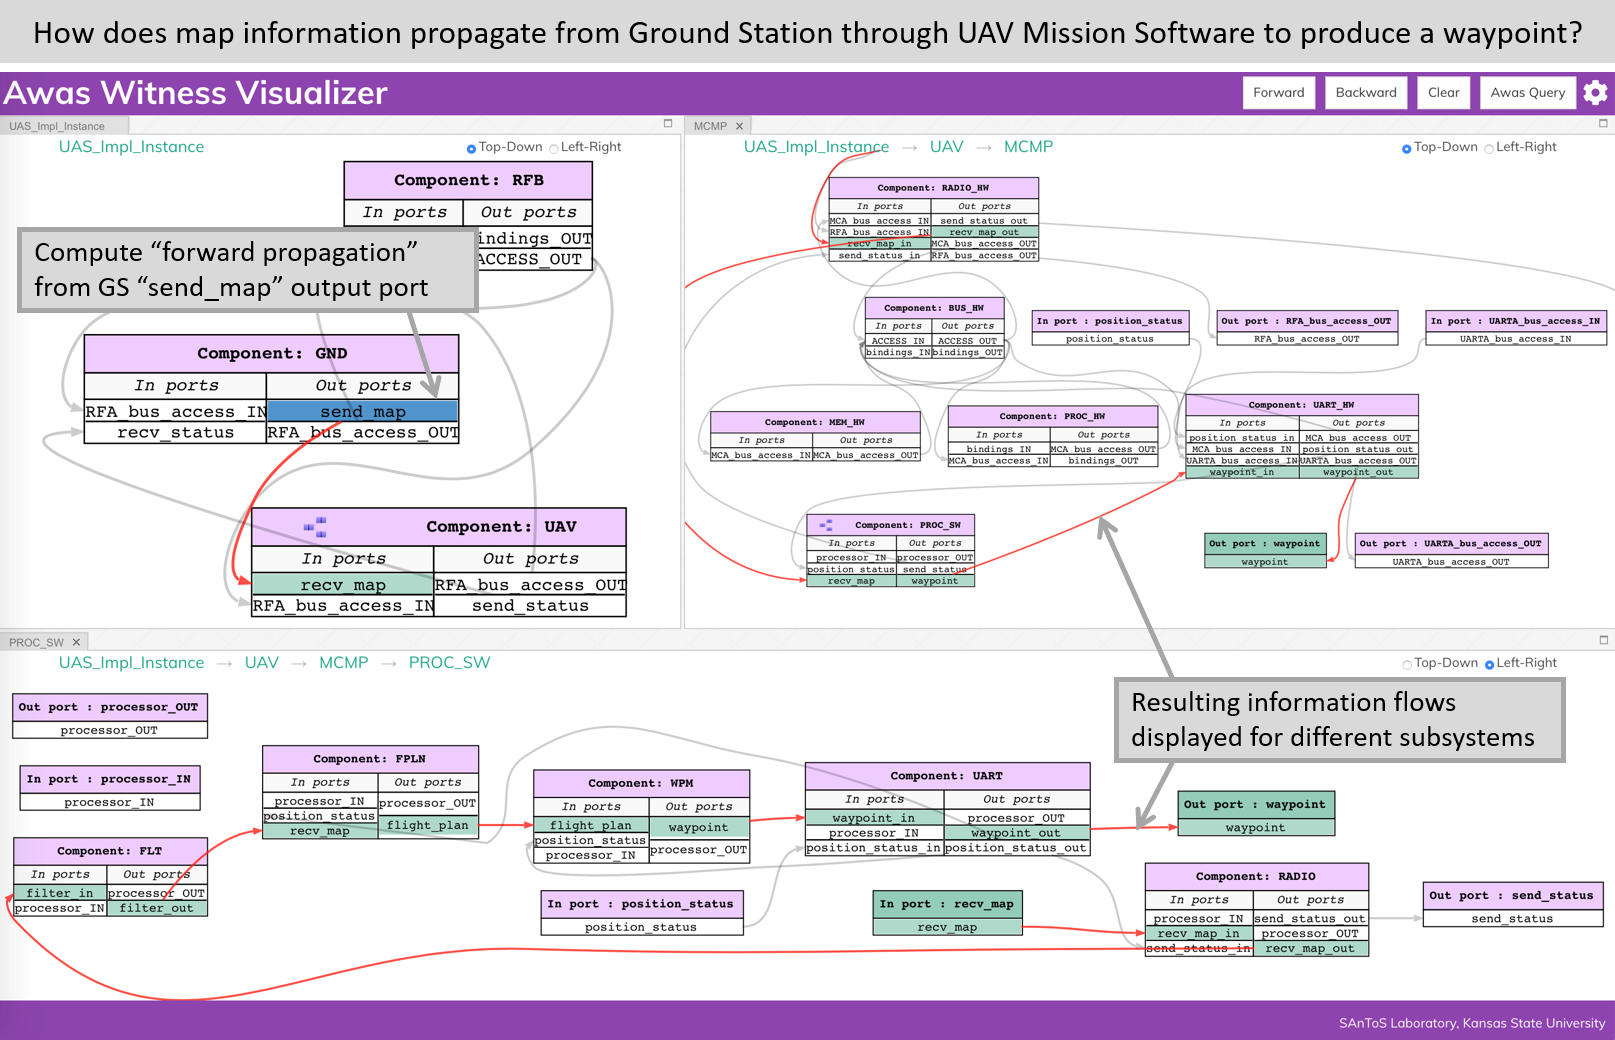
\includegraphics[width=\textwidth]{figs/CASE-Awas.png}
	\caption{Awas Information Flow Analysis.} 
	\label{fig:CASE-Awas} 
\end{figure*}

Figure~\ref{fig:CASE-Awas} illustrates an example of Awas information flow reachability analysis.
%From a given component or port (e.g., an output port of the Ground Station),
In our UAV example, Awas can compute and visualize how the information in Ground Station messages flows through the system
as well as the components or ports that may directly or indirectly consume data derived from that information.
Awas supports a number of forms of forward and backward interactive information queries.
Using the Awas script-based query language, one can specify and check more complex properties, e.g.,
that information must flows through specific ports or components.
These end-to-end flow specifications are often useful for supporting verification of the
effectiveness of cyber-resiliency components.   An Awas specification can state that
information from untrusted components such as the Ground Station always flow through the
Attestation Gate and filter components before reaching the Flight Control or other components
that make critical decisions about the flight or mission of the UAV.

%The HAMR code generation and associated formally verified information
%flow correspondence evidence described subsequently
%%%described in Section~\ref{subsec:hamr}
%guarantees that the seL4 microkernel is configured to permit the exact
%inter-component information flows analyzed and visualized by Awas at
%the model level.


\subsection{Real-Time Scheduling}
%John S -  Budget: 1 column
% Real-Time Scheduling

In mixed-criticality mission systems,
execution threads often 
have strict confidentiality, integrity, and availability requirements. 
Under certain conditions,
timing channels can be manipulated to violate these security requirements. 
For example, temporal interference between timing channels
can reduce availability of time-critical functionality 
and weaken the integrity of controls by inducing selective jitter.
As a result, a compromised component could dominate the processor, 
preventing other components from completing their tasks, placing the security 
of the entire platform in jeopardy. 
Simple scheduling approaches that attempt to use priority schemes to mitigate 
this impact only protect the highest priority threads and leave the other
threads vulnerable.

\emph{Temporal isolation} is a more secure technique to restrict timing channels and
reduce temporal interference between software threads executing on the same platform. 
\briefcase\ achieves temporal isolation by leveraging
prior work from safety and security-critical disciplines, such as
avionics, where temporal isolation in real-time scheduling has been
deployed for decades.
We implemented a static cyclic scheduling
approach using the \selFour\ domain scheduler, where a fixed schedule
defines an ordered sequence of static execution slots. Each slot has a
duration and a partition identifier.  \selFour\ ensures that the
temporal domain, and any threads running in it, will not exceed their defined
time allotments. Thus, each thread executes within its own
well-defined timing constraints without interference from other threads.
System designers are responsible for the
creation of a valid static cyclic schedule that
satisfies all the application's timing requirements.

\briefcase\ generates a start-of-frame synchronization signal for each thread using
a special thread called the Pacer, which sends periodic signals
to each thread. Each application thread blocks until it receives its
signal from the Pacer. The application thread runs to completion, and then
blocks again on the Pacer signal for the next iteration. 
Each thread subsequently executes
exactly once during its statically scheduled time slice.

The new \selFour\ Mixed-Criticality Systems (MCS) variant provides
additional capability that can support temporally isolated
real-time systems. 
As part of \briefcase\ we developed a proof-of-concept static cyclic
scheduler for MCS.
It includes a start-of-frame signal, which
eliminates the need for the Pacer component. It also includes kernel
level support for flexible dynamic scheduling that satisfies some
real-time properties, such as period and execution time.



\subsection{Infrastructure Code Generation}
% John H -  Budget: 1 column
\label{subsec:hamr}

%% Text for the Infrastructure Code Generation subsection
% - assigned to John Hatcliff

HAMR \cite{hamr} is a multi-platform, multi-language
AADL code generation framework.  On CASE, HAMR is primarily used
to generate code for deployment for the seL4 microkernel, but system and component
prototyping is also supported utilizing HAMR's code generation capability
for the Java Virtual Machine (JVM) and Linux.  For seL4 deployments, one of the
primary CASE-inspired objectives is to generate system builds that
leverage seL4 micro-kernel partitioning and information flow
controls to achieve the AADL-specified component separation and
inter-component communication needed to support cyber-resiliency.

For each AADL thread component, HAMR generates a thread code
skeleton and APIs for communicating over the ports declared on
the component.  For components that are implemented directly, the
developer fills out the thread skeleton with application code,
calling the port APIs, libraries, and component-specific
developer-implemented support code as needed.
HAMR supports coding component application logic in either C,
Slang~\cite{slang} (a high-assurance subset of Scala that can be translated to
C), or CakeML.  Slang-implemented components can interface with
Scala or Java libraries and executed on the JVM.  Pure Slang
components can be translated to C and then deployed on HAMR-built
Linux or seL4 systems.  On CASE, Slang has been used for prototyping
components, but primary development of directly implemented
components have used C.  For high-assurance components specified
using SPLAT, HAMR automatically integrates code generated from
SPLAT into the component binary code using CakeML's Foreign
Function Interface (FFI) mechanism.

HAMR generates component infrastructure and integration code
implementing the semantics of AADL-compliant thread scheduling,
thread dispatching, and port-based communication.
For port communication, both shared memory communication (AADL
data ports), buffered messaging (AADL event data ports), and
buffered notification (AADL event ports) are supported.
HAMR code generation is staged using a translation architecture
that facilitates adding new backends for different target
platforms.   Almost all the infrastructure code is implemented
in Slang, which can then be used for JVM deployments or
translated to C for Linux or seL4 deployments.
The Slang-based implementation of the AADL run-time framework
can be viewed as a high-level reference implementation of AADL
semantics.   Automatic translation of this reference
implementation to C on different platforms helps establish
semantic consistency across different platforms. 
CASE formal methods such as the AGREE contract language and SPLAT
code generation framework are designed to align with the AADL
semantics reflected in the reference implementation.  

To generate deployments on seL4, HAMR makes heavy use of the
CAmkES code-generation framework.   The CAmkES input
language is a domain-specific language that supports specification
of seL4 partitioning and communication topology using
component-oriented idioms.  The CAmKES translator generates an
seL4 \emph{Capability Description Language (CapDL)} file that
configures the seL4 kernel to support protected memory blocks
and permission-based reading and writing of each block as
indicated by CAmkES components and connections.
To realize the spatial separation specified by the AADL
architecture description, HAMR generates CAmkES specifications
that: (a) reflect the AADL model's component and communication
topology, and (b) include additional components and communication
to support the AADL run-time infrastructure, in particular,
thread scheduling.
HAMR also provides automated support for configuring Linux-based
virtual machines as components within the seL4 deployed system. 
In CASE, this feature has been used to sandbox untrusted legacy code.
To enforce time partitioning, HAMR uses the seL4 \emph{domain
scheduler} to suport static scheduling.  In CASE workflows,
the FASTAR AADL scheduling tool from Adventium Labs was used
to generate a candidate static schedule, and then the schedule
was adjusted as needed based on timing experiments (this was
needed primarily for VM components).

HAMR-generated seL4 deployments can be executed on the Qemu ARM
hardware simulator before deployment to a development board or
production hardware.  This significantly sped up development
iterations and enabled the development of a sophisticated
automated regression testing framework.

While CASE scope did not include full formal verification of
the HAMR Slang-based reference implementation and code generation
pipeline, the Collins CASE team selected the key property of
information flow preservation to illustrate how one might build
out to formal verification of important semantic properties.
Specifically, HAMR generates flow graphs reflecting the
inter-component information flow at both the AADL architecture
level and the seL4 CAmkES level.  In addition to multiple
visualizations and auditable traceability artifacts, HAMR
generates SMT-based representations of the flow graphs and
traceability relationships between them.  Formalized
theorems for information flow preservation can then be represented as
SMT assertions.  This enables SMT solvers to automatically prove
the following properties for any HAMR-generated seL4 deployment:
(a) [All AADL flows realized] For every inter-component information
flow present in the AADL model, that flow is provisioned in the
generated seL4 kernel configuration;  (b) [No extraneous flows] For
each inter-component flows provised in the seL4 kernel, that
flow is represented as an inter-component connection in the
AADL model.   This property was chosen to emphasize the
cyber-resiliency dimension of the CASE program, but other
key semantic properties of the AADL run-time can be incrementally
formally verified, e.g., by applying the Slang Logika formal
verification capability to the Slang reference implementation of the
AADL run-time.  

Overall, HAMR plays a key role in integrating formal methods
at different levels of abstraction at multiple points throughout
the development process, enabling those methods to be applied
at-scale in a DoD system development process.   Using the
formally verified seL4 microkernel as a foundation, HAMR enables
AADL to be used as a model-based development and systems
engineering framework for seL4-based applications.
HAMR provides a semantically-consistent multi-platform code
generation process that enables: (a) formally verified components
(e.g., generated from SPLAT) to be correctly integrated and
deployed; and (b) formal specification and verification frameworks
like AGREE to be used to reason about both component and system
level properties.   The HAMR code generation architecture is
designed to support strong traceability and verification, and
the CASE program has illustrated how key properties such as
information flow correspondence properties can be established
via formal verification.   The compositional and staged nature
of HAMR-based development enables scaling of formal approaches
by enabling them to be included in a targetted fashion --
component-wise and at different levels of abstraction -- while
also integrating parts of the implementation that are assured
using traditional methods.   In addition, the strong partitioning
of seL4 enables the controlled integration of untrusted components.





\subsection{Secure Microkernel}
% Corey, Gerwin -  Budget: 1 column
% word budget: ~ 400 words

The seL4 microkernel is a lightweight, fast, and secure operating system (OS) kernel.
Its implementation is fully formally verified from high-level security properties
down to the binary level~\cite{sel4-formal}. It was the first OS kernel with this
degree of formal verification, and after more than a decade of further research
and engineering is still not only the leading formally verified OS kernel, but also
the fastest OS kernel on the Arm architecture.

Its formal verification makes seL4 the ideal basis for high-assurance systems.
It is in itself a demonstration of the level of fidelity and scale formal
verification can achieve. It supports multiple architectures (Arm, x86-64,
RISC-V), deep security properties such as integrity, confidentiality and
availability, it comes with formally verified user-level system initialization,
and as one of multiple available OS personalities, it offers a user-level component
system that provably achieves isolation between statically specified components.

The formal proofs about seL4 and the corresponding user-level components measure
over one million lines of proof script in total. They constitute one of the
largest continually maintained formal proof artifacts in existence and provide a
rich target for new techniques in proof engineering, proof repair, and
automation for constructing new proofs about software as well maintaining
existing large-scale proof artifacts.

While it is essential to build a high-assurance system on a high-assurance OS
kernel, this is not the main feature seL4 provides for systems engineering --- a
simpler real-time OS may well be formally verified, but not be sufficient for the
engineering method described in this paper. The true power of seL4 lies in its
ability to scale formal analysis and verification to the much larger code bases
that make up the entire system. It does so by providing strong isolation between
user-level components.

This isolation means that components can be analyzed separately from each other
and be composed safely --- seL4 provides the basis for the soundness of the highly
automated analysis tools such as AGREE can provide. It makes it possible to run
entire untrusted virtual machines and securely monitor their behavior on the
same hardware. It makes it possible to provide filter and monitor components and
prove that these components cannot be tampered with by the components they protect.
It makes it possible to ensure that the communication channels the analysis tools
assume are the \emph{only} communication channels that are available to the
components in the system.


\subsection{Assurance Case}
%Isaac -  Budget: 1 column
An important aspect of our work on CASE has been to structure formalizations and proofs by following the AADL description of the system. In other work, we did this through the use of formal assume-guarantee contracts that correspond to the requirements for each component~\cite{HACMS}. We have found that in assuring the cyber-security properties of aircraft designs we need to integrate different kinds of evidence with varying levels of formality. This has been our motivation to explore assurance case methods.

In previous work, we developed the {\em Resolute} language and tool~\cite{resolute2014},~\cite{resolute-destion} as a way to help developers create an assurance argument describing the steps taken during the design process to make the system safe and secure.  
The Resolute syntax supports construction of assurance cases that comply with the Goal Structuring Notation (GSN) v2 standard~\cite{GSNv2}.  Claims are expressed as \textit{goals} and \textit{strategies}, and can contain attributes such as \textit{context}, \textit{assumptions}, and \textit{justification}.  Claims can be marked \textit{undeveloped}, which Resolute interprets as an unsupported claim, or with a \textit{solution}, which is an explicit assertion that the claim is supported.
Rather than being a separate document, a Resolute assurance case is part of the architecture model and can refer to elements within the model. Since it is not a static representation, it can ensure that the assurance argument remains consistent with the evolving design.

BriefCASE includes a library of Resolute assurance strategies, or \textit{patterns}, that align with the CASE workflow.  The patterns are instantiated with context from the AADL model, and specify the evidence required to support the cyber-resiliency goals of the system.  
%
For example, the \texttt{add\_filter} strategy is automatically inserted into the assurance case when the \textit{Filter} transformation is performed, and includes logical rules that Resolute uses to determine whether the well-formedness claim is  supported by evidence.
The \texttt{add\_filter} definition (shown in Figure~\ref{fig:resolute-add-filter}) includes the following sub-goals: 
\begin{itemize}
	\item \texttt{filter\_exists} - the filter component exists in the model
	\item \texttt{filter\_not\_bypassed} -  there is no alternate pathway in the model that can bypass the filter
	\item \texttt{filter\_implemented\_correctly} - the filter has been implemented correctly
\end{itemize}


\begin{figure}[h]
	\centering
	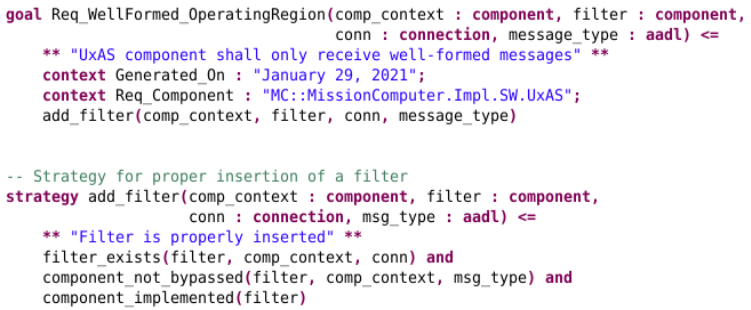
\includegraphics[width=1\columnwidth]{figs/resolute-add-filter.png}
	\caption{Updated well-formedness claim.} 
	\label{fig:resolute-add-filter} 
\end{figure}

The first two sub-goals are supported by evidence obtained by examining the structure of the model, while the last is determined by examining the output of the synthesis tool.  
If at a later time during development the model is inadvertently altered in a way that renders the transformation ineffective, Resolute will be unable to substantiate the evidential statements, and therefore produce a failing assurance case.

The third subgoal is satisfied by SPLAT.  SPLAT not only generates the implementation code for high-assurance components such as filters, monitors, and gates, but it also produces a proof that the generated code correctly implements its AGREE specification.  
Resolute uses the existence of the SPLAT proof as evidence that the component was implemented correctly.


% Resolute can determine whether an assurance case passes or fails


% Advocate?

% Show generated assurance case (in Advocate?)

\section{AIRCRAFT APPLICATION}
%David -  Budget: 1 column
Collins Aerospace has successfully demonstrated the CASE methodology and tools on the CH-47F Common Avionics Architecture System (CAAS), utilizing a team of CAAS development engineers.  As an integrated cockpit avionics suite, CAAS serves as a prime example of modern air platform complexity with common avionics across a variety of defense platforms including the Army�s Mission Enhanced Little Bird (MELB) and MH-60, the Navy CH-53K, and the Air Force  KC-135.  As the primary designer and manufacturer of CAAS, Collins Aerospace maintains complete design artifacts including boot loaders, operating systems, software applications, hardware, and bus message specifications.  CAAS offered an opportunity to apply CASE tools across a variety of mission systems including legacy components, flight critical software, as well as new and evolving systems.

Our primary goal was to enable CAAS product engineers to employ the CASE tools to create an operational mission scenario  exhibiting cyber threats and mitigations that could be exercied using the facilities of the Collins CH-47F System Integration Laboratory.  The CH-47F demonstration system for CASE focused on three areas: integrating pilot and soldier wireless tablet computers for increased situational awareness, detecting  attempted Automatic Dependent Surveillance (ADS-B) traffic spoofing, as well as porting the high-assurance seL4 operating sytem to an existing Collins CAAS product processing module.  This processing module, or VPM, is provisioned to allow only vetted traffic to/from the aforementioned wireless clients in order to provide situational awareness data to pilots and soldiers, as well as to provide a platform for the execution of CASE-tool-generated filters, monitors, attestation gates, etc.

The CAAS developers first developed an AADL model of the CH-47F CAAS system.  They then added the enhanced capabilities described above, resulting in a baseline architecture.  The CAAS development engineers then analyzed their baseline AADL architecture utilizing the GearCASE and DCRYPPS tools, resulting in a set of cyber requirements.  They then employed the BriefCASE AADL plug-in to provision filters, monitors, attestation gates, seL4 isolates, etc., in order to satisfy the cyber requirements.  The specifications for the filters and monitors were developed by the CAAS developers using the AGREE contract language, with assistance from the CASE developers, and the SPLAT tool was invoked by BriefCASE in order to synthesize the monitors and filters from the AGREE specifications with high assurance, as described previously.  The HAMR tool was then invoked by BriefCASE in order to synthesize the overall system, including the seL4 CAmkES components, CAmkES I/O, the processing schedule, etc.

The tablet operating environment utilized either an off-the-shelf Android environment, or a Linux guest OS running on seL4.  This provided the CASE remote attestation team with differing challenges when it came to the measurement and attestation of the tablet platform types, and provided the CASE independent evaluators a variety of options for formulating attacks against the system.  The ADS-B anti-spoofing monitor developed by the CAAS team detected position/velocity trend inconsistencies, duplicate traffic identifiers, as well as ``teleporting'' aircraft.

The port of the seL4 microkernel to the Collins VPM product was complicated by the need for network proxy/adapters to bridge the untrusted wireless network to the rest of the sytem in a trustworthy manner, including the ability to filter encrypted network traffic payloads.  Fortunately, dedicated processing cores were available on the VPM for the provisioning of these low side and high side proxy/adapters.  This code had to be manually generated due to the complexity of dealing with off-the-shelf networking technologies; automating the synthesis of network adapter/proxy components is future work.  

The CAAS developers experienced tool immaturity/expressiveness/documentation issues, as was to be expected for the first use of a research tool suite by product area developers.  Initial estimates of processing time required to run the monitoring components turned out to be overly optimistic, requiring an optimization effort.  Lack of detailed seL4 support for the target hardware led to more extensive porting efforts for the VPM and tablets than was originally anticipated, and tablet hardware instabilities further hampered the porting effort.  But all in all, the CASE tools were able to be productively used by Collins product area engineers to produce the CH-47F CAAS demonstration system on time and within budget, providing the CASE developers with valuable feedback on the strengths and weaknesses of the current CASE tool envionment.



\section{CONCLUSION}
% Budget: 0.5 column
%The manuscript should include a conclusion. In this section,
%summarize what was described in your paper. Future directions may
%also be included in this section. Authors are strongly encouraged not
%to reference multiple figures or tables in the conclusion; these
%should be referenced in the body of the paper.
We have produced a model-based systems engineering environment
called BriefCASE, based on the Architecture Analysis and Design
Language.  The BriefCASE tools and methodology provide design, analysis, and code
generation capabilities based on formal methods and targeted at
high-assurance cyberphysical systems.  

Key innovations include automated architectural design patterns 
for cyber-resiliency, co-evolution of system design and assurance 
artifacts (captured as an assurance case linked to the architecture model), 
synthesis of code for high-assurance components, and code generation
targeting the formally verified seL4 microkernel.  

We have demonstrated the effectiveness and scalability of these 
tools by using them to add new cyber-resilient features to a military 
helicopter avionics system.  Their successful use by our product engineers 
provides evidence that formal methods can be incorporated into 
industrial projects.  

All of the tools are open-source, with links and documentation available
at \url{http://loonwerks.com/projects/case.html}.  We hope that others 
will find value is this approach and extend the tools with new cyber transforms, 
expanded system analysis tools, and code generation for additional operating 
systems and computing platforms.  







%BriefCASE provides
%access to two cyber requirements analysis tools (GearCASE
%and DCRYPPS) that can examine AADL models to detect potential
%cyber vulnerabilities and suggest requirements for mitigation.
%A library of architectural transforms guides systems engineers
%through automated model transformations that modify the
%architecture to address these requirements, oftentimes inserting new
%high-assurance components synthesized from formal
%specifications using the SPLAT tool. Formal verification that the
%transformed system model satisfies its cyber requirements is accomplished
%via model checking using the Assume Guarantee Reasoning
%Environment (AGREE). Cyber-resilient code implementing the
%verified model is automatically generated using the HAMR
%tool. If desired, this code can be targeted to the formally
%verified seL4 secure microkernel.  Another novel aspect of our approach is
%the use of an assurance argument embedded in the architecture model
%itself to capture and document the design decisions made during this
%process, along with associated rationale.
%
%We have successfully demonstrated our BriefCASE methodology and tools on the
%CH-47F helicopter Common Avionics Architecture System (CAAS), utilizing a team of CAAS
%development engineers who had no previous experience with formal methods.  We
%are currently incorporating lessons learned from this experience to improve the BriefCASE
%methodology and tools, focusing on scalability and usability.


%open-source, prototype, extensible to other domains
%link to loonwerks.com
%significance -- recap innovations, scale, accessibility
%application to real systems

\section{ACKNOWLEDGMENT}

This work was funded by DARPA contract HR00111890001. The
views, opinions and/or findings expressed are those of the authors
and should not be interpreted as representing the official views or
policies of the Department of Defense or the U.S. Government.

\bibliographystyle{IEEEtran}
\bibliography{biblio}

\begin{IEEEbiography}{Darren Cofer}{\,}is a Fellow at Collins Aerospace. His research interests include formal methods and tools for verification and certification of high-integrity systems. He received his PhD in Electrical and Computer Engineering from the University of Texas at Austin and is a senior member of the IEEE. Contact him at cofer@ieee.org.
\end{IEEEbiography}

\begin{IEEEbiography}{Isaac Amundson}{\,}is a research engineer at Collins Aerospace, focusing on MBSE, formal verification and assurance.  He received his PhD in Computer Science from Vanderbilt University.
\end{IEEEbiography}

\begin{IEEEbiography}{Junaid Babar}{\,}is a researcher at Collins Aerospace.
Do not fold, spindle, or mutilate.  
\end{IEEEbiography}

\begin{IEEEbiography}{David Hardin}{\,}is a research engineer
  at Collins Aerospace, and has made contributions in
  the areas of formal methods, high-assurance computer architecture,
  and real-time embedded Java.  He is editor of the book \emph{Design
    and Verification of Microprocessor Systems for High-Assurance
    Applications}.  He received a PhD in Electrical and Computer
  Engineering from Kansas State University.
\end{IEEEbiography}

\begin{IEEEbiography}{Konrad Slind}{\,} (PhD, TU Munich) is an industrial logician at Collins Aerospace.
  His research interests include design and implementation of higher
  order logic theorem provers, verified compilation, and
  self-describing data formats.
\end{IEEEbiography}

\begin{IEEEbiography}{Perry Alexander}{\,}is the AT\&T Foundation
  Distinguished Professor and Director of The Information and
  Telecommunication Technology Center at The University of Kansas.
  His research interests include trusted computing, remote
  attestation, formal verification and formal synthesis. He received
  his PhD from The University of Kansas.
\end{IEEEbiography}

\begin{IEEEbiography}{John Hatcliff}{\,}
John Hatcliff is a University Distinguished Professor and
Lucas-Rathbone Professor of Engineering in the Computer Science
Department at Kansas State University.  His research interests include
software architecture, formal verification, and interoperability in 
the avionics, automotive, and medical domains.
He received his PhD in Computer Science from Kansas State University.
\end{IEEEbiography}

\begin{IEEEbiography}{Robby}{\,}
is a Professor of Computer Science at Kansas State University working
in the area of formal methods, software engineering, and programming
languages.
%%He received his PhD in Computer Science from Kansas State University.
He received a NASA Turning Goals Into Reality award in 2003,
a NSF CAREER award in 2007, an ICSE 2000 Most Influential Paper award in 2010,
and an ACM SIGSOFT Impact award in 2010.
\end{IEEEbiography}

\begin{IEEEbiography}{Gerwin Klein}{\,}
is Chief Scientist at Proofcraft and Conjoint Professor at UNSW Sydney. His
research interests include software verification, semantics of programming
languages, and proof engineering. He is the architect of the seL4 microkernel
verification which received the SIGOPS Hall of Fame Award. He received his PhD
in Computer Science from TU Munich.
\end{IEEEbiography}

\begin{IEEEbiography}{Corey Lewis}{\,}%
  is a Senior Proof Engineer at UNSW Sydney. He has been involved in all stages
  of the verification of the seL4 microkernel.
\end{IEEEbiography}

\begin{IEEEbiography}{Eric Mercer}{\,}
  is an Associate Professor at Brigham Young University.
  His research interests include software verification, model checking, static analysis, and programming languages.
  He received his PhD in Electrical Engineering from the University of Utah.
\end{IEEEbiography}

\begin{IEEEbiography}{John Shackleton}{\,}
  is a Senior Principal Research Scientist at Adventium Labs,
  focused on real-time embedded systems, cybersecurity, and
  model-based system engineering and analysis.
\end{IEEEbiography}

%Author's latest degree received or which he/she is currently pursuing
%(He received the B.S. degree and the M.S. degree...."). Author's
%research interest. Association with any official journals or
%conferences; major professional and/or academic achievements, i.e.,
%best paper awards, research grants, etc.; any publication information
%(number of papers and titles of books published). Author membership
%information, e.g., is a member of the IEEE and the IEEE Computer
%Society, if applicable, is noted at the end of the
%biography. Biography is limited to single paragraph only (He is a
%member of IEEE, etc.). All biographies should be limited to one
%paragraph, five to six sentences


\end{document}
